\documentclass[11pt, a4paper]{article}

\usepackage{graphicx}
\usepackage[english]{babel}
\usepackage[utf8x]{inputenc}
\usepackage{amsmath}
\usepackage{amssymb}

\usepackage[a4paper,top=3cm,bottom=2cm,left=2cm,right=2cm,marginparwidth=1.75cm]{geometry}
\graphicspath{ {./images} }

\begin{document}

\setcounter{section}{1}
\section{Lecture 2 (13/02/2020)}

\subsection{Dynamics of pulley mechanisms}
Analyzing the dynamics of pulley mechanisms will raise some interesting questions.
Say there is a pulley mechanism as shown in figure 1 below. At what velocicty would mass A
move upwards as a result of pulling mass B downwards. Intuition tells us that these velocities
are indeed different but by what factor? Setting up just the equations of motion does not solve this problem
since there are 2 equations with 3 variables. This is an unsolveable system. 
The following example will discuss techniques that can be applied in analyzing the geometry of these kinds of systems
to create an extra constraint equation to solve the system. The constraint equation represents a
boundary under which the system can excist as described.

\subsection{Example problem involving pulleys}
\begin{figure}[h]
    \centerline{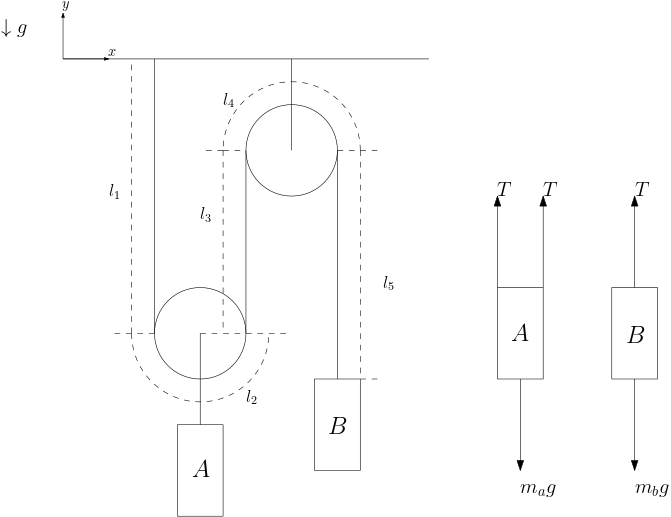
\includegraphics[width=10cm]{images/Pulleys.png}}
    \caption{Free Body Diagram of the Pulley mechanism to be analyzed for the example}
\end{figure}

\begin{align}
    \Sigma F_{ay} = 2T - m_a g = m_a \ddot{y}_a \\
    \Sigma F_{by} = T - m_b g = m_b \ddot{y}_b
\end{align}
\\
Note that the problem has 3 unknown variables ($T$, $\ddot{y}_a$ and $\ddot{y}_b$).
There are only 2 equations of motion, which would make this system of equations
unsolveable. To correct for this a third eqaution is introduced.
The rope is divided into 5 lengths. When mass b is moved downwards $l_5$ gets longer.
mass a moves upwards which means $l_3$ and $l_1$ both get shorter.
Since the total length of the cable does not change\footnote{Mechanics of materials tells us that the length does in fact change
as a result of tension in the rope, but since this deformation is much smaller then
the total length of the rope it's not worth considering this elongation.}.

\begin{equation}
    l_t = l_1 + \cdots + l_5 \Leftrightarrow l_t = \sum_{i=1}^{5} l_i
\end{equation}

We can conclude that the length of $l_2$ and $l_4$ does not change since the size
of the pulleys does not magically change. The total length must also stay constant
since it's still the same rope. The rate of displacement and rate of change in velocity
of the parts of the ropes are also equal to one another because the equality holds when both
sides of an equation are derrived. It is also know that the change in velocity of $l_1$ and $l_3$
must be equal to $\ddot{y}_a$ but in opposite direction. This also holds
for $l_5$ and $\ddot{y}_b$.

\begin{gather}
    f(x) = g(x) \\
    \frac{d}{dx} \Big(f(x) - g(x)\Big) = 0 \Rightarrow f'(x) = g'(x)
\end{gather}

From this we can conclude that:

\begin{gather}
    l_t = \sum_{i=1}^{5} l_i \Leftrightarrow \ddot{l}_t = \sum_{i=1}^{5} \ddot{l}_i \\
    \ddot{l}_t = 0 \qquad \ddot{l}_1 = -\ddot{y}_a \qquad \ddot{l}_2 = 0 \qquad \ddot{l}_3 = -\ddot{y}_a \qquad \ddot{l}_4 = 0 \qquad \ddot{l}_5 = -\ddot{y}_b
\end{gather}

subsituting equation (7) into equation (6) will give the following:
\begin{gather}
    0 = -\ddot{y}_a +  -\ddot{y}_a +  -\ddot{y}_b\\
    \ddot{y}_b = -2\ddot{y}_a
\end{gather}

Equation (9) is the constraint equation. This equation determins the condition under which
the system is consistent with itself. There are now 3 variables and 3 equations making this system solveable.

\subsection{Vectors and their properties}
Much like calculus, linear algebra proves to be a powerfull tool for solving dynamics problems.
Examples of this are expressing forces as a vector and equations of motion as systems of equations.
Some important properties of vectors will be listed below. These include vector addition, vector multiplication 
with cross- and dotproduct and some general algebraic rules for manipulating vectors. All defenition are given in 3D space.
Since this is the most common use for use of vectors in mechanics, since physical real space has 3 dimensions.

\setcounter{equation}{0}
\begin{gather}
    \vec{r}_b = \vec{r}_a + \vec{r}_{b/a} \\
    c \vec{a} = ca_1\boldsymbol{\hat{i}} + ca_2\boldsymbol{\hat{j}} + ca_3\boldsymbol{\hat{k}}\\
    \vec{a} \cdot \vec{b} = a_1 b_1 + a_2 b_2 + a_3 b_3 = |\vec{a}||\vec{b}|\cos(\theta)\\
    \vec{a} \times \vec{b} = (a_2 b_3 - a_3b_2) \boldsymbol{\hat{i}} + (a_3 b_1 - a_1 b_3)\boldsymbol{\hat{j}} + (a_1 b_2 - a_2 b_1)\boldsymbol{\hat{k}}\\
    |\vec{a} \times \vec{b}| = |\vec{a}|\vec{b}||\sin(\theta)
\end{gather}

Also note that the accelaration vector ($\vec{a}$) has some interesting properties when considering
circular motion. The vector can be split up is 2 components. 1 tangential to the circular motion
which could be considered the instantaneous accelaration and 1 perpendicular to that towards the center
of the circle. This is the apparant cetrifugal force in circular motions. More on this topic will 
discussed in a later lecture.
\newpage

\subsection{State dependent accelaration}
Consider the velocity and accelaration as described by a derrivative. Note that both
of these are time dependent. In some cases a dynamical system is described by it's current state\footnote{The state
of any dynamical system is it's posistion and velocity, it's accelaration is not part of the state.}
rather then by the passage of time (example: $a=kv^2$, $a = ks$, where $k$ is some random constant). It is usefull 
for cases like this to have an equation which describes the accelaration in terms of velocity rather then time. 
Note that a mathematician would probably shoot me for the "derrivation"\footnote{Treating infitesimals as fraction is mathematically considered
bad practice since it can lead to nonsensical math such as $\Big(\frac{dy}{dx}\Big)^2 = \frac{(dy)^2}{(dx)^2}$. That being said the notation does allow for
fraction-like manipulations that are in fact correct (such as $f'(x) = \frac{df(x)}{dx} \Leftrightarrow f(x) = \int f'(x)\,dx$). The real derrivation for
$ads = vdv$ would be far more rigoureus.} 
I am about to give but it works for all intents of purposes.

\begin{gather}
    a = \frac{dv}{dt} \qquad v = \frac{ds}{dt} \\
    dt = \frac{dv}{a} \qquad dt = \frac{ds}{v} \\
    \frac{dv}{a} = \frac{ds}{v}\\
    ads = vdv \Leftrightarrow a = v\frac{dv}{ds}
\end{gather}

Note that in equation (9) $\frac{dv}{ds}$ is the derrivative of velocity with respect to displacement.
If v is constant equation (9) can be further reduced as follows:

\begin{gather}
    \int a\,ds = \int v \, dv \\
    \int a\,ds = \frac{1}{2}v^2
\end{gather}

\end{document}